\section{Robustness and participant heterogeneity}\label{sec:heterogeneity}
\subsection{Source conditions and repeat seeds}
Checkpoint quality also varied before target access. On source-validation participants, checkpoint-mean BA ranged from 50.00\% to 78.36\% for EEGNet and 50.00\% to 72.82\% for the Conformer. Those participants contributed to checkpoint selection. The ranges provide context for the frozen conditions and cannot establish out-of-sample source performance.

Figure~\ref{fig:source_omission} holds the target cohort and prefix-ten policy fixed. At each spoke we omit one training condition from the summary of existing checkpoints. For each seed, we average gains over the four retained conditions within each participant, then over the same 62 Stieger2021 participants. All ten cross-seed omission means are positive. Positive leave-one-condition-out averages do not imply positive gains for every individual source condition. On the same 62 participants, the Conformer trained on BNCI2014-001 alone averaged $-0.323$ points across its three seeds. Two Conformer seed means fall just inside the zero ring. Omitting LODO gives $-0.08$ points at seed 17, and omitting Lee2019-MI gives $-0.04$ at seed 43.

\begin{figure}[t]
\centering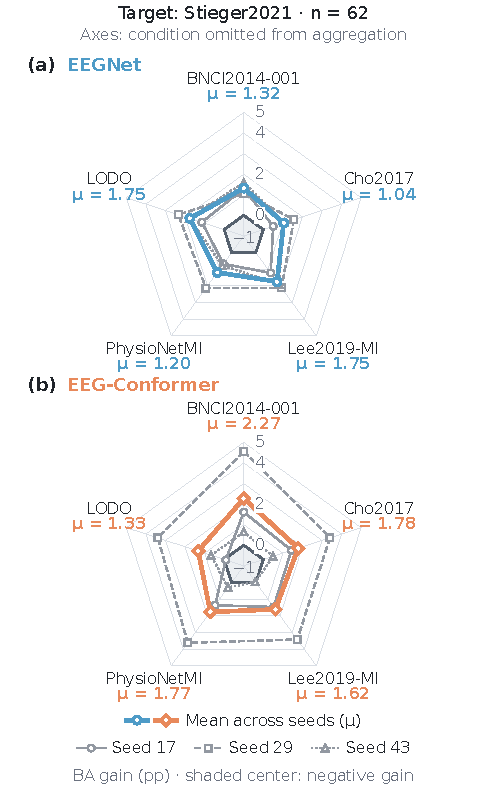
\includegraphics{figures/figure4_source_robustness_radar.pdf}
\caption{Training-source omissions on the protected Stieger suffix. Every spoke omits the named training condition from aggregation, with all checkpoints frozen. LODO denotes the multi-source condition. Gray contours describe seeds 17, 29 and 43. The colored contour and $\mu$ labels give their mean. Both panels use the same linear scale from $-1$ to $+5$ BA points. The bold zero ring encloses negative gains. Seed contours convey no confidence interval. Performance comparisons use spoke values and exclude polygon area.}\label{fig:source_omission}
\end{figure}

The participant bootstrap asks how the mean would vary with the participant sample at this fixed model grid. A second weighting first averages participants within each training condition and resamples the five condition means. The resulting gain intervals widen to [0.40, 2.42] points for EEGNet and [0.60, 2.75] for the Conformer. Dataset-balanced weighting equals participant weighting on a single external dataset. None of these intervals measures variation across newly trained backbones or unobserved acquisition sites.

\begin{table}[t]
\caption{Between-seed Spearman correlations of participant gain on the protected suffix. For each backbone and seed, gains are averaged over all five training conditions before ranking the same 62 participants.}\label{tab:robust}
\centering\small\begin{tabular}{@{}lrr@{}}\toprule
Seed pair & EEGNet & Conformer \\\midrule
17 vs. 29 & 0.70 & 0.77 \\
17 vs. 43 & 0.57 & 0.31 \\
29 vs. 43 & 0.82 & 0.44 \\
\bottomrule\end{tabular}
\end{table}

Table~\ref{tab:robust} shows how consistently the seeds rank participants by gain. Agreement varies especially for the Conformer, from 0.31 to 0.77. Participants, training conditions and seeds recur across the omission contrasts.

\subsection{Oracle transfer across sessions}
\begin{figure}[t]
\centering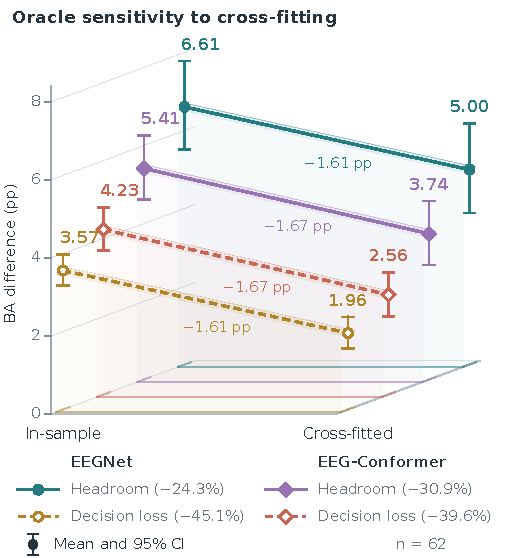
\includegraphics{figures/figure6_oracle_sensitivity.pdf}
\caption{Oracle sensitivity on complete eligible Stieger sessions. The in-sample threshold uses all eligible trials of a participant. Cross-fitting predicts each held session using labels from the other sessions. Decisions from the held sessions are pooled for BA on the same complete records. Points and whiskers are means and marginal 95\% participant intervals ($n=62$). Connecting segments show point changes. Relative reductions use the corresponding in-sample mean.}\label{fig:oracle}
\end{figure}

The leave-one-session-out replay evaluated 17,760 model--participant--session folds across the 30 models. Each participant contributed at least two eligible sessions and no model-session fold was excluded. Moving the threshold fit off the held session reduced EEGNet decision loss from 3.57 to 1.96 points and Conformer loss from 4.23 to 2.56 (Fig.~\ref{fig:oracle}). The corresponding held-session 95\% intervals were [1.56, 2.38] and [2.00, 3.13] points. Mean headroom fell from 6.61 to 5.00 [3.89, 6.19] points and from 5.41 to 3.74 [2.94, 4.58]. These estimates provide a reference for transferring a threshold across sessions, including sessions later in acquisition order. Subtracting the protected prefix gain would mix different sets of trials.

\subsection{Counting at a fixed model}
\begin{figure}[t]
\centering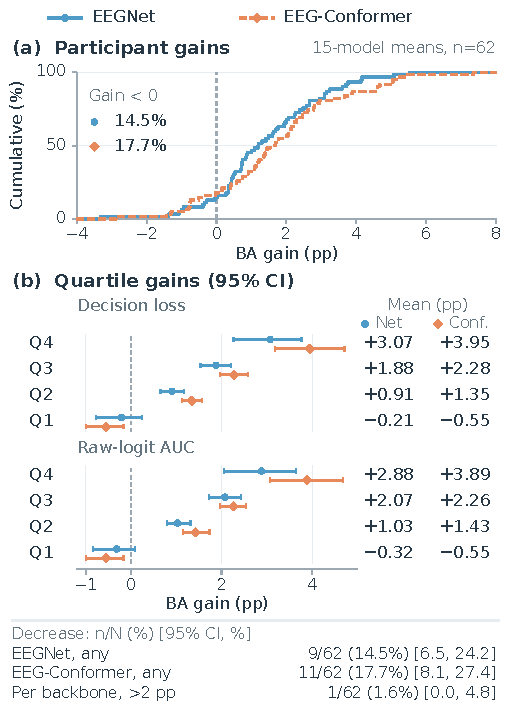
\includegraphics{figures/figure7_participant_degradation.pdf}
\caption{Participant gains on the protected suffix after averaging 15 source-condition/seed configurations within each participant and backbone. (a) Empirical cumulative distributions and fractions below zero. The footer gives the resulting participant counts and rates for each backbone. (b) Mean gains and 95\% participant intervals by within-backbone decision-loss or AUC quartile. Quartile sizes are 16, 15, 15 and 16. Intervals condition on the original membership. The same participant can occupy different quartiles across stratifiers and backbones.}\label{fig:strata}
\end{figure}

The median participant gain after averaging models was 1.19 points for EEGNet and 1.62 for the Conformer. Nine and eleven of the 62 participants, respectively, had negative averages. Each backbone had one participant with a decrease exceeding two points, or 1.6\%. The original percentile interval for this rare count is 0.0--4.8\%. A Wilson sensitivity gives 0.3--8.6\%, conditional on the observed classifications. With one event, neither interval gives a stable upper bound on the risk to a future individual.

For a fixed checkpoint, we instead counted participants with gain strictly below $-2$ BA points before aggregating across models. Using the same 62 participants for every checkpoint, EEGNet's 15 counts ranged from 1/62 to 14/62, compared with 1/62 after averaging. The 15 Conformer counts ranged from 0/62 to 17/62, also compared with 1/62 after averaging. No model was selected using these counts. They describe retrospective heterogeneity conditional on model identity.

Figure~\ref{fig:strata} locates the negative tail after model averaging. Each curve contains one gain per participant. In the lowest AUC quartile, mean gains were $-0.32$ and $-0.55$ points, with 8/16 and 11/16 participants below zero. In the highest AUC quartile the means rose to 2.88 and 3.89 points. The decision-loss quartiles show a related gradient. Gain and decision loss share the default BA term, and the in-sample oracle constrains recoverable gain for a static policy. These strata use outcomes from the evaluated suffix and cannot select participants in advance. A positive cohort mean, seed-to-seed agreement and the degradation count for a named checkpoint convey distinct evidence about transfer.
